\section{Example Conservative Forces}
\subsection{Gravitational Force Near the Earth's Surface}
As shown in the previous section, the gravitational force near the Earth's surface is given by
$$\underline{F} = m\underline{g} = -mg\underline{k}$$
where $m$ is the {\bf mass} of the object and $\underline{g}$ is the {\bf gravitational acceleration} near the Earth's surface. \\
And therefore we can derive the following:
$$\begin{aligned} -mg\underline{k} & = \Big(\underline{i}\frac{\partial}{\partial x} + \underline{j}\frac{\partial}{\partial y} + \underline{k}\frac{\partial}{\partial z} \Big)(-mgz) \\ \\
                                 & = -\underline{\nabla}(mgz)\end{aligned}$$
Therefore we can define the following:
\begin{definition}[Gravitational Potential Energy Near the Earth's Surface]
	The {\bf gravitational potential energy} $\Phi$ is given by:
	\begin{equation}
		\label{eq: gravitational-potential-energy-near-earth}
		\Phi = mgz
	\end{equation}
\end{definition}

\begin{eg}[Calculating Velocity]
	A particle is dropped from rest at a height $z=h$.
	Calculate the velocity

		{\bf Solution:} \\
	We know that the particle is dropped from rest, therefore $\underline{v} = 0$ at $t=0$ at height $z = h$ Therefore.

	$$E = K + \Phi = \frac{1}{2}m\mid\underline{0} \mid^{2} + mgh = mgh$$
	At height $z = 0$, height is 0 so
	$$E = K + \Phi = \frac{1}{2}m\mid\underline{\dot{r}}\mid^{2} + mg0 = \frac{1}{2}m\mid\underline{\dot{r}}\mid^{2}$$
	Since {\bf Energy is a constant}, we get that:
	$$\begin{aligned} mgh = \frac{1}{2}m\mid\underline{\dot{r}}\mid^{2} & \Rightarrow 2gh = \mid \underline{\dot{r}}\mid^{2}     \\ \\
                                                                  & \Rightarrow \mid \underline{\dot{r}} \mid = \sqrt{2gh}\end{aligned}$$
\end{eg}

\subsection{Gravitational Potential Energy Away from the Earth's Surface}
Consider the following diagram:
\begin{mycenter}



	\tikzset{every picture/.style={line width=0.75pt}} %set default line width to 0.75pt        

	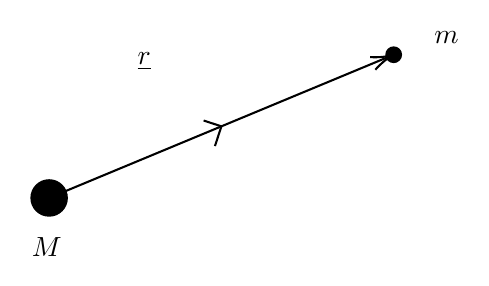
\begin{tikzpicture}[x=0.75pt,y=0.75pt,yscale=-1,xscale=1]
		%uncomment if require: \path (0,300); %set diagram left start at 0, and has height of 300

		%Shape: Circle [id:dp3521186394752994] 
		\draw  [fill={rgb, 255:red, 0; green, 0; blue, 0 }  ,fill opacity=1 ] (124.3,194.53) .. controls (124.3,189.82) and (128.12,186) .. (132.83,186) .. controls (137.55,186) and (141.37,189.82) .. (141.37,194.53) .. controls (141.37,199.25) and (137.55,203.07) .. (132.83,203.07) .. controls (128.12,203.07) and (124.3,199.25) .. (124.3,194.53) -- cycle ;
		%Shape: Circle [id:dp673844600958276] 
		\draw  [fill={rgb, 255:red, 0; green, 0; blue, 0 }  ,fill opacity=1 ] (295.3,125.53) .. controls (295.3,123.58) and (296.88,122) .. (298.83,122) .. controls (300.78,122) and (302.37,123.58) .. (302.37,125.53) .. controls (302.37,127.48) and (300.78,129.07) .. (298.83,129.07) .. controls (296.88,129.07) and (295.3,127.48) .. (295.3,125.53) -- cycle ;
		%Straight Lines [id:da15576096830380182] 
		\draw    (132.83,194.53) -- (296.99,126.3) ;
		\draw [shift={(298.83,125.53)}, rotate = 157.43] [color={rgb, 255:red, 0; green, 0; blue, 0 }  ][line width=0.75]    (10.93,-3.29) .. controls (6.95,-1.4) and (3.31,-0.3) .. (0,0) .. controls (3.31,0.3) and (6.95,1.4) .. (10.93,3.29)   ;
		%Shape: Right Angle [id:dp6024123881050093] 
		\draw   (207.28,157.24) -- (215.83,160.03) -- (212.73,169.54) ;

		% Text Node
		\draw (317,113) node [anchor=north west][inner sep=0.75pt]   [align=left] {$\displaystyle m$};
		% Text Node
		\draw (174,123) node [anchor=north west][inner sep=0.75pt]   [align=left] {$\displaystyle \underline{r}$};
		% Text Node
		\draw (123,212) node [anchor=north west][inner sep=0.75pt]   [align=left] {$\displaystyle M$};


	\end{tikzpicture}
\end{mycenter}

The gravitational potential energy is given by:
$$
	\begin{aligned}
		\underline{F} = m \underline{\ddot{r}} & = -\frac{mMG}{\mid \underline{r}\mid^{2}} \frac{\underline{r}}{\mid \underline{r} \mid } \\ \\
		                                       & = -\underline{\nabla}\Big(-\frac{mMG}{\mid \underline{r}\mid}\Big)                       \\ \\
	\end{aligned}
$$
\begin{definition}[Gravitational Potential Away From Earths Surface]
	The {\bf gravitational potential} $\Phi$ is given by:
	\begin{equation}
		\label{eq: gravitational-potential-away-from-earth}
		\Phi = -\frac{mMG}{\mid \underline{r}\mid}
	\end{equation}
\end{definition}
